\section{Model}

This section describes the underlying model and ideas for the $\Phi_{ASE}$
calculation in an active gain medium with planar top and bottom surfaces (see
figure \ref{graphic:samples_reduced}).



\subsection{The crystal mesh} \label{subsec:meshSampling}

To distribute the \emph{sample points} on the medium, it is seen as a
horizontal 2-dimensional plane, which can be sampled with a non-uniform
density. This approach allows to increase the spatial resolution in certain
areas of interest. Using Delauny triangulation, these sample points are
connected to a 2D mesh of triangles.

The triangle mesh is extruded in direction of the vertical axis to form a
\emph{slice} of right prisms (figure \ref{graphic:extruded_mesh}). This
slice is then duplicated several times, until the whole medium is divided into
prisms (figure \ref{graphic:samples_reduced}).

\begin{figure}
  \centerline{
    \resizebox{0.45\textwidth} {!} {\includegraphics{graphics/delauny_3.png}}
  }
  \caption{extruded plane of triangles}
  \label{graphic:extruded_mesh}
\end{figure}

\begin{figure}
  \centerline{
    \resizebox{0.45\textwidth} {!} {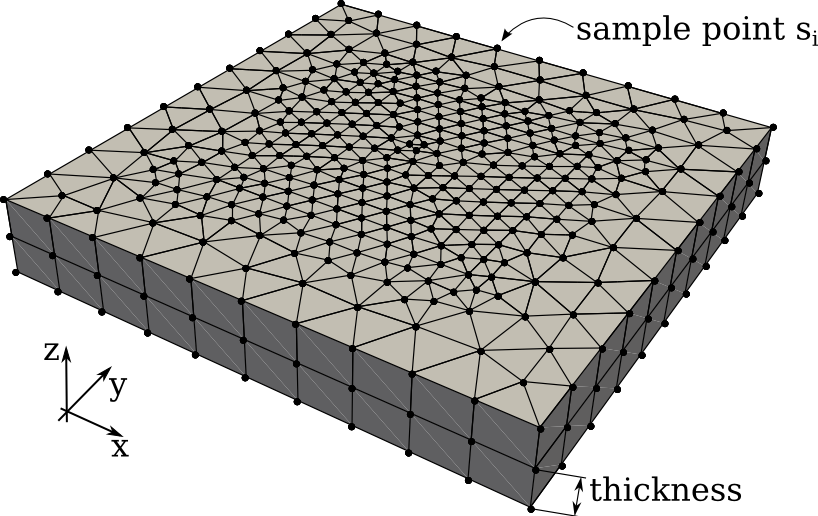
\includegraphics{graphics/samples_reduced.png}}
  }
  \caption{non-uniform sampling of active gain medium in 2 slices}
  \label{graphic:samples_reduced}
\end{figure}




\subsection{Ray tracing}
\label{subsec:raytracing}

To calculate the amplification of a single ray from a position $r_i$ to a sample
point $r_0$, the ray is traced along its path through the prisms (see figure
\ref{graphic:prism_propagation}). 

\begin{figure}[H]
  \centerline{
    \resizebox{0.45\textwidth} {!} {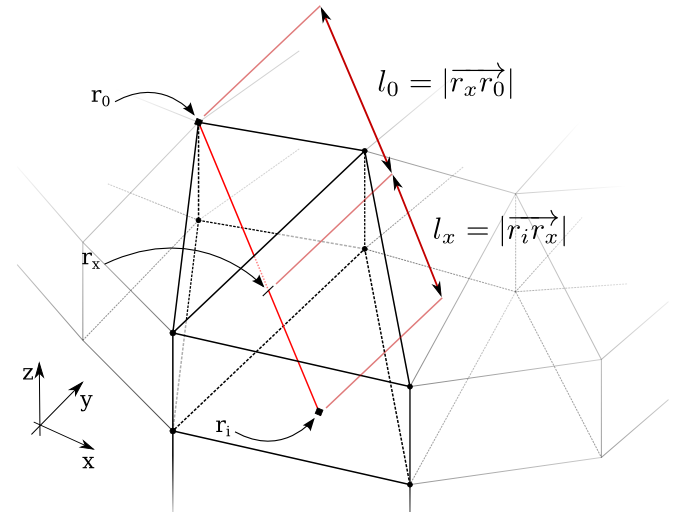
\includegraphics{./graphics/prism_propagation_2.png}}
  }
  \caption{propagation of a ray through the prism structure}
  \label{graphic:prism_propagation}
\end{figure}

Starting from point $r_i$ inside a prism, there are 5 possible intersection
planes for the ray. One plane for the top and bottom surfaces and one for each
of the 3 horizontal sides. Once the intersection plane is determined (the ray is
intersecting at point $r_x$), the next prism can be calculated based on the
knowledge about the meshing structure:

\begin{description}

  \item[horizontal side]
    the ray will remain in the same slice, but the next prism is based on a
    different triangle. This triangle is a \emph{neighbor} of the previous one.
    The relevant datastructure to determine the neighboring triangle is created
    during the Delauny triangulation in \ref{subsec:meshSampling}.

  \item[top/bottom plane]
    if the ray is intersecting with the top or bottom plane of the prism, the
    next prism will be based on the same triangle as before, but in a different
    slice.

\end{description}

This process is iterated for each prism on the path between $r_i$ and the
desired sample point $r_0$. The intersections (like $r_x$) with prism surfaces
define line segments of a certain length $l_x$. These segments are used for the
gain calculation: For each prism $x$, the contribution to the gain is calculated
as a function of $l_x$:
\[ 
  partial\_gain(x) = 
  e^{N_{tot} \cdot (\beta_x \cdot (\sigma_e + \sigma_a) - \sigma_a)) \cdot l_x}
\]
where $\beta_x$ is the \textbf{TODO: describe beta} beta value in the current
prism.

The gain for the whole ray can then be computed as
\[ 
  gain(\overrightarrow{r_ir_0}) =  
  \frac {\beta_i}  {dist(r_i,r_0)^2 }
  \cdot 
   \prod^n partial\_gain(n) 
 \]



\subsection{Reflections}
\label{subsec:reflections}

In order to allow for reflecting rays on the upper and lower surface of the medium, the model is
extended to include the refractive indices of the medium and the surrounding.
Furthermore, each triangle on the surfaces may be covered with a different coating
material.  



\begin{itemize}

  \item Depending on the material and coating, there are different
    reflectivities on the crystal's surfaces.

  \item A fast simulation allows to take reflecting rays into account and to
    estimate the impact of lateral lasing.

  \item Only reflections on upper and lower plane implemented until now.

\end{itemize}



\subsection{Monte Carlo simulation}
\label{subsec:monteCarlo}

\begin{itemize}

  \item \textit{integral is expressed by formula} \cite[Daniel's Thesis]{ASE2010}

  \item Monte Carlo simulation as a way to calculate the integral for the whole
    crystal.

  \item \textit{formula for the additive Monte Carlo}

\end{itemize}






